\chapter{Основная часть}
\section{Имеющиеся данные}
В рамках программы SAHR были записаны ЭКГ (использовалось только первое отведение) 1800 москвичей преклонного возраста (55-91 год). Из них 46\% мужчин. Запись каждого ЭКГ производилась в течение суток. В это же время за человеком велось дополнительное наблюдение и было известно, в какой промежуток времени он спал, а в какой - бодрствовал. Также про каждого человека известна некоторая информация: состояние здоровья, вес, курит ли он и многое другое.
\section{Постановка задачи}

Цель работы - анализируя данные ЭКГ предсказать в какое время человек спал/бодроствовал, исследовать возможность предсказания болезней и самочувствия человека.Также в рамках обучени выделения признаков и их анализа были проведены исследования по идентификации человека.

\section{Актуальность задачи}
Электрокардиография - самый распространенный клинический инструмент, который измеряет электрическую деятельность сердца с поверхности тела. Сигнал ЭКГ, или проще вариабельности сердечного ритма содержит много интересной информации о человеке. Сейчас медицинские институты в дополнение к существующим базам данных (SAHR, AHA DB, ESC DB и т. д.) формируют новые. Также разработано множество новых технологий и приборов, таких как фитнесс-браслеты, специальные чехлы для телефонов, мониторы-холтеры и др., позволяющих человека без каких либо трудностей и специального медицинского оборудования круглосуточно (или в любое удобное для него время) записывать информацию о своем пульсе. Для врачей повилась возможность постоянно контролировать состояние пациента и отправлять их данные  для анализа и отчетности. Популярность подобных носимых устройств для мониторинга здоровья растет с каждым годом. Они позволяют человеку быть подвижным, заниматься своими делами и в это же время собирать данные о своем здоровье в "естественной" среде. Точность этих приборов уступает специализированным установкам - но даже по их сигналу можно многое сказать о человеке. 

Качество и длительность сна имеют важное значение для медицинской диагностики []. Однако на практике сложность процедуры классической полисомнографии [] накладывает существенные ограничения для ее применения. Несмотря на множество информации, которую предоставляют носимые электронные устройства и исслдеований в этом направлении, на сегодняшний день нет хороших научных доказательств, представленных публике, о том, что они могут оценить продолжительность сна с высокой точностью.

\section{Фильтрация ЭКГ сигнала и выделение RR-пиков}
\subsection{Фильтрация ЭКГ}
Сигнал ЭКГ, собираемый носимыми устройствами, подвержен влиянию множества шумов. На него могут влият следующие причины, никак напрямую не связанные с сердцем.
\begin{itemize}
	\item Погрешности устройства
	\item Неплотное прилегание устройства к коже
	\item Подвижность человека (сокращения мыщц, и др.)
	\item Физические реакции, не связанные с рердечной деятельность (к примеру, внезапные сокращения мыщц при засыпании)
\end{itemize}
%Иногда сигнал с устройства выглядит следующим образом. рис.


\subsection{Выделение RR-пиков}
Для определения R-пиков данный сигнал обрабатывался рядом фильтров. На первом этапе нам наиболее важно выделить найти местоположение R-пиков и не имеет значения, какой вид примет QRS-комплекс. Фильтрация производится на основе дискретного преобразования Фурье (ДПФ): проводится ДПФ, зануляются нужные коэффициенты и производится обратное преобразование ДПФ. Какие именно коэффициенты занулять «подсмотрено» в сторонних библиотеках Matlab для анализа кардиограмм.

Вид сигнала после применения фильтров можно наблюдать на рис.  \ref{ris:filter_ekg}

\begin{figure}[h]
	\begin{minipage}[h]{0.47\linewidth}
		\center{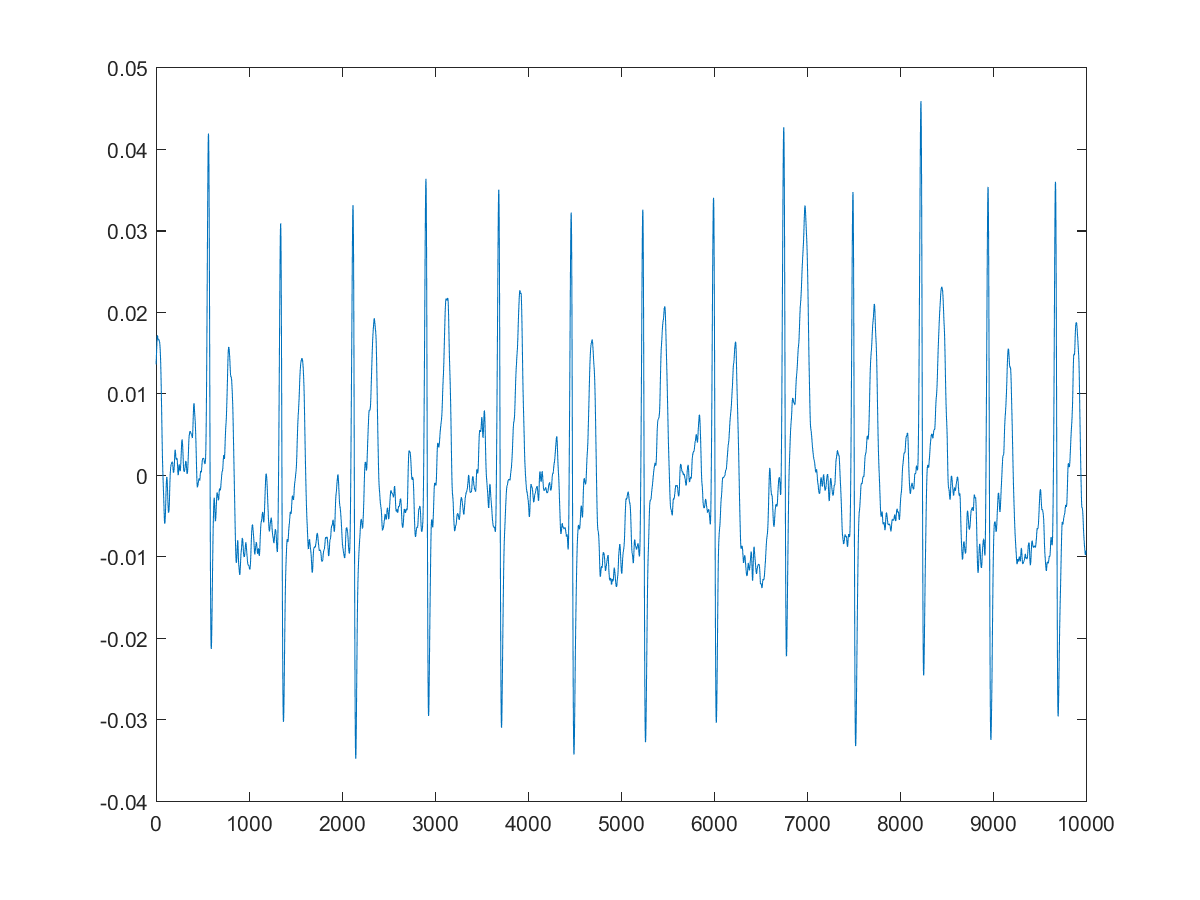
\includegraphics[width=1\linewidth]{filtered_ekg_base}} a) \\
	\end{minipage}
	\hfill
	\begin{minipage}[h]{0.47\linewidth}
		\center{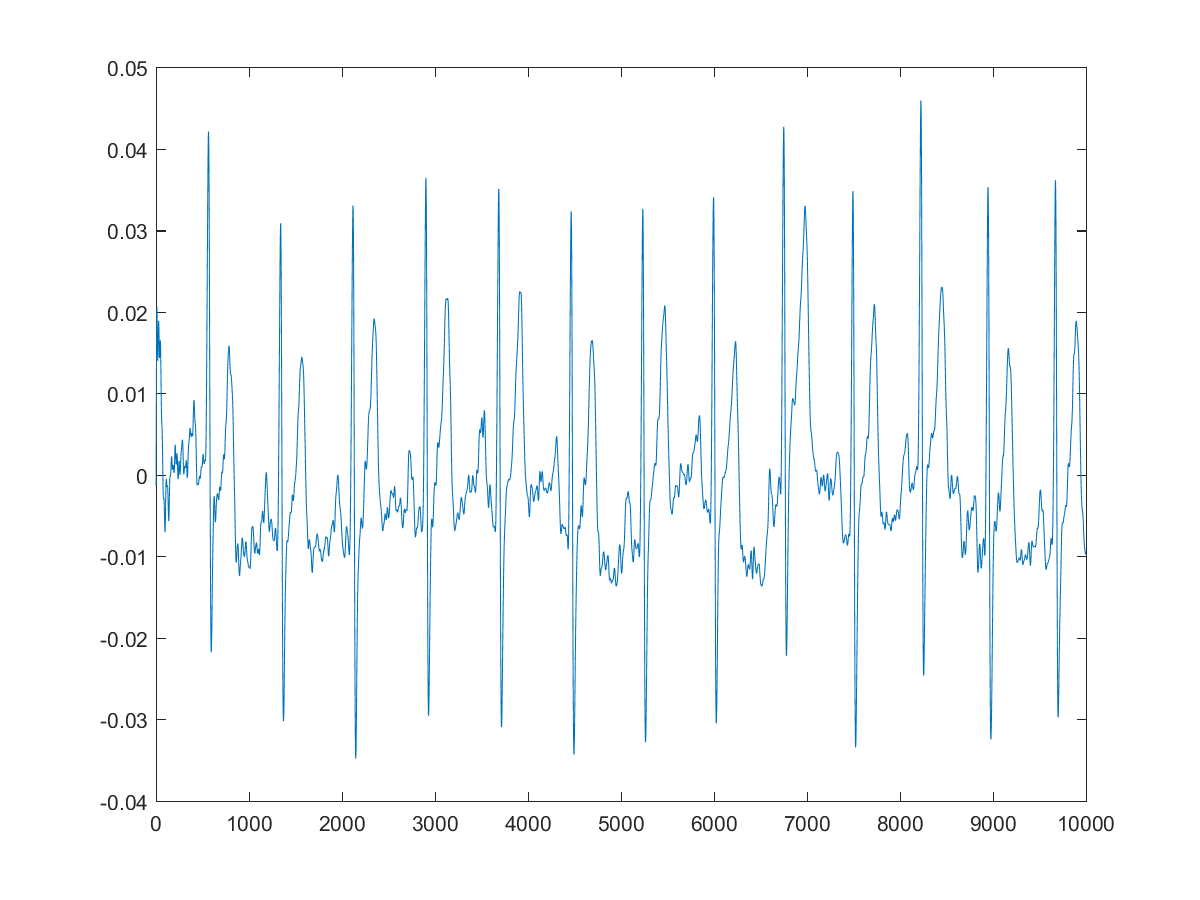
\includegraphics[width=1\linewidth]{filtered_ekg_hig}} \\b)
	\end{minipage}
	\vfill
	\begin{minipage}[h]{0.47\linewidth}
		\center{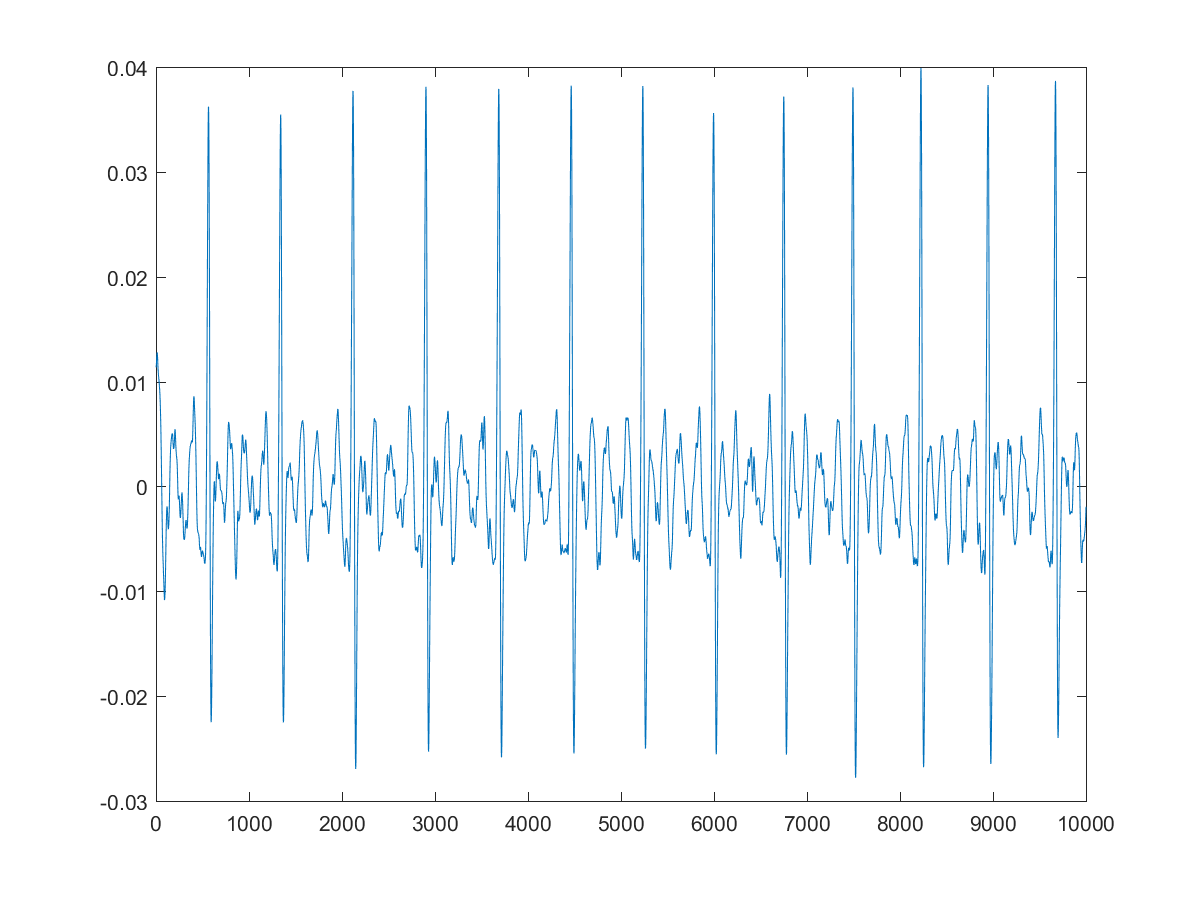
\includegraphics[width=1\linewidth]{filtered_ekg_low}} c) \\
	\end{minipage}
	\hfill
	\begin{minipage}[h]{0.47\linewidth}
		\center{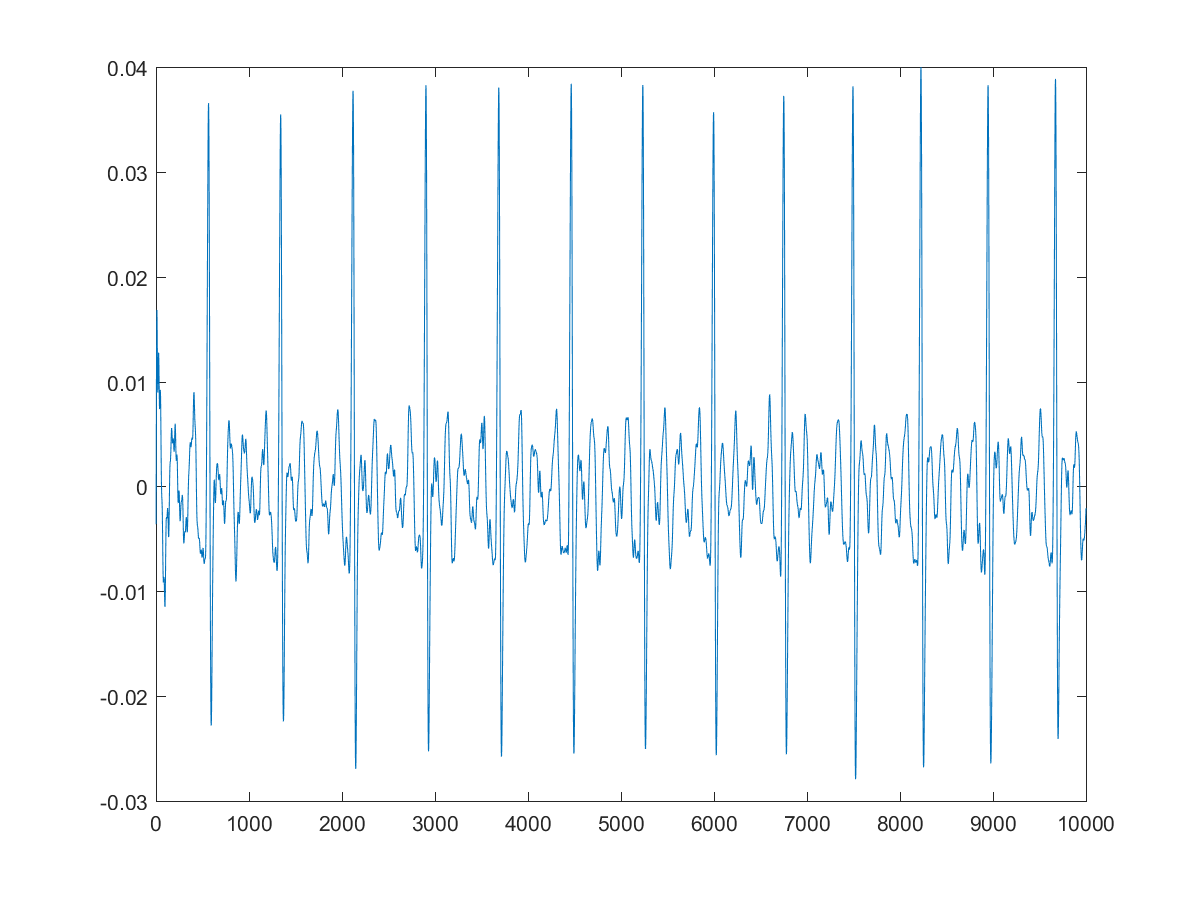
\includegraphics[width=1\linewidth]{filtered_ekg_low_hig}} d) \\
	\end{minipage}
	\caption{ЭКГ сигнал a)до фильтрации b) после высокочастотного фильтра
		c) после низкочастотного фильтра d) после обоих фильтров}
	\label{ris:filter_ekg}
\end{figure}

Для определения RR-пиков отбирались точки $i$ такие, что $x_i$ - локальный максимум в окне $[x_{i-k\_pred}, ..., x_i,    , x_{i+k\_next}]$, а также $min([x_{i-r\_pred}, ..., x_i])<0$ и $min([x_i, ..., x_{i+r\_next}])<0$. То есть сигнал справа и слева от локального минимума опускается ниже нуля. Напомню, что мы работаем с фильтрованным сигналом, среднее значение которого лежит около нуля.

Далее, когда мы определили координаты пиков на фильтрованном сигнале - находим обратным преобразванием их на исходном. Признаки, считаемые по QRS-комплексу считались по неотфильтрованныму сигналу, дабы не потерять информацию. Фильтр низких частот, применение которого желательно при поиске пиков, очень сильно искажает сигнал. 
QRS-комплекс размечался по следующему алгоритму:
статья дьяконова
код никиты - ссылки из него
картинки найденного QRS-комлекса

\section{Работа с RR-сигналом}
\subsection{Отбор RR-пиков}
При снятии сигнала возникают лишние пики. Они могут быть вызваны сокращениями мыщц, резкими движениями или другими различными причинами. При не очень плотном прилегании электрода какой-то кусок сигнала может быть потерян. При первичной обработке сигнала вырезались длительные участки сигнала без пиков (если на протяжени 2 минут не было пиков), и выкидывался участок сигнала между пиками, расположенными ближе чем 200 мс.

примеры плохого сигнала

Для классификации промежутков времени на сон/бодрствование необходим весь временной ряд. Но для идентификации человека, для предсказания каких-либо характеристик достаточно только его части. Если брать для предсказания характеристик небольшие участки сигнала размер обучающей выборки увеличится в несколько раз, увеличится ее обобщающая способность.

То, что мы берем только участки сигнала позволяет нам отобрать участки с минимумом шума. На сигнал могут влиять случайные движения человека, непроизвольные сокращения мыщц. Может быть не очень хорошо закреплен электрод или же он может сдвинуться или отойти на время. в первом случае мы получаем лишние пики, во втором, наоборот, долгий промежуток без них. 

Было решено отбирать участки сигнала где все выделенные R-пики удовлетворяют следующим условиям:

\begin{itemize}
	\item разница высот соседних пиков менее 20\%
	\item разница продолжительностей соседних RR интервалов менее 20\%
\end{itemize}

\subsection{Выделение признаков}
Большая часть подсчитываемых признаков по выделенным R пикам описана в обзоре литературы - они являются стандартными при работе в ЭКГ сигналом. Однако вдобавок к ним использовались еще добавочные признаки.
\begin{itemize}
	\item амплитуды пиком и минимумов в QRST-комплексе
	\item разница высот между пиками P, R, T
	\item отношения ввысот P, R, T
	\item средние значения на промежутках PQ, QR, QT
	\item длительнисть различных фаз в QRST-комплексе
	\item площадь под графиком на промеежутках PQ, QS, ST, begin-Q, S-final
\end{itemize}
В медицине утверждается [!! ссыдки], что врачи ориентируются на данные параметры при постановки диагноза.
\section{Проведенные экперименты}

В рамках данного исследовая проводились попытки решения следующих задач.
\subsection{Идентификация человека}
Люди делились на 3 выборки: тестовую, валидационную и обучающую. Экг каждого человека нарезались на отрезки. Состовлялись пары отрезков, для каждой пары устанавливалось из одного сигнала они взяты (1) или из разных (0). Далее пары отрезков подавались на вход сети :
 архитектуру? надо ли вообще. я об этом так себе знаю - это твое исследование было
Качество предсказания на тестовом датасете - 75\%. Количество элементов каждого класса во всех выборках было равным.
\subsection{Предсказание сна}
Предсказание сна - актуальная задача по следующим причинам (из литобзора).
В ходе данного исследования эта задача решалась следующими методами.
\subsubsection{Линейный классификатор}
Если смотреть на RR-сигнал во время сна и бодроствования (одну картинку сюда - сделать красиво) можно заметить, что во время сна частота пульса уменьшается (достаточно очевидное ,предположение известное всем). Также можно заметить уменьшение дисперсия сигнала во время сна.
Первым предложенным алгоритмом был следующий.
\begin{enumerate}
	\item для сигнала подсчитывались среднее значение и дисперсия
	\item маркируются все точки сигнала на три категории
	\begin{itemize}
		\item точки на половину дисперсии больше среднего значения
		\item точки на половину дисперсии меньше среднего значения
		\item все остальные точки (формулой бы?)
	\end{itemize}
	\item Далее мы ищем наиболее длинную последовательность точек из первой группы, не прерываемую более чем 5 точками из второй в лоюбом ее месте
\end{enumerate}
Количество точек было подобрано на обучающей выборке. (исправить - посмотреть, сколько точно)
Качество предсказания - 75\%.
Картинок сюда.
\subsubsection{Деревья}
Далее было принято решение увеличить количество признаков и кроме среднего и дисперсии посчитать стандартные приз
Далее было решено проверить следующее предположение: при работе с RR сигналом люди считают множество признаков - может быть не просто так. Давайте посчитаем их и на них что-нибудь обучим.
\subsection{Предсказание болезней}